\documentclass[conference]{IEEEtran}

\usepackage{cite}
\usepackage{amsmath,amssymb,amsfonts}
\usepackage{algorithmic}
\usepackage{graphicx}
\usepackage{textcomp}
\usepackage{xcolor}
\usepackage{verbatim}
\usepackage[brazilian]{babel}
\usepackage[utf8]{inputenc}
\usepackage[T1]{fontenc}

% \def\BibTeX{{\rm B\kern-.05em{\sc i\kern-.025em b}\kern-.08em
%     T\kern-.1667em\lower.7ex\hbox{E}\kern-.125emX}}
\begin{document}

\title{Análise Comparativa da Aplicação de Filtros Digitais no Controle Gear VR}
%\title{Visualização do Filtro de Kalman na Estabilização de Controle para Realidade Virtual}

\author{\IEEEauthorblockN{Thiago Figueira\IEEEauthorrefmark{1},
Adriano Gil\IEEEauthorrefmark{1}}
\IEEEauthorblockA{\IEEEauthorrefmark{1}Samsung Instituto de Desenvolvimento para a Informática da Amazônia\\
SIDIA,\\
Manaus -- AM -- Brazil}}

\maketitle

\begin{abstract}
Kalman filter is a digital filter capable of predicting, with high precision, past, present and future states given a linear dynamic system with Gaussian noise. Even though an effective tool, Kalman filter is not a built-in implementation in Unity3D development environment. Therefore, this paper intends to implement  a visualization tool in which the Kalman filter is applied to a noisy virtual reality device joystick. It's also an objective to explain how the filter works as well as present the results of its use.
\end{abstract}

\begin{IEEEkeywords}
virtual reality, games, digital filters
\end{IEEEkeywords}

%Reescrever mais
\section{Introdução}
% 1. Contextualizar o problema
Jogos e aplicações de realidade virtual utilizam \textit{hardware} especial para permitir a interação do usuário através de sensores inerciais - tais quais o acelerômetro, giroscópio e magnetômetro - os quais mensuram orientação, aceleração, taxa angular, campos magnéticos e essencialmente traduzem um evento na realidade do usuário para seu correspondente no cenário virtual.

Estes sensores têm a finalidade de quantificar comportamentos ou características da realidade através de transdutores que convertem a energia de entrada em energia de saída. Neste processo, registra-se uma amostra do evento de interesse, isto é, processa-se uma série de capturas da realidade de maneira a converter a medida de interesse em um conjunto contínuo de valores. Este procedimento, contudo, está suscetível a erros, seja devido à natureza física do transdutor que não traduz fielmente os valores medidos, seja na insuficiência dos dados capturados pela amostragem, ou ainda na discretização dos valores contínuos da realidade. Somadas estas possibilidades, percebe-se que as informações de interesse (velocidade, orientação, localização no GPS, etc.) são suscetíveis a ruídos, isto é, o valor medido não reflete em sua totalidade a verdadeira condição do sistema no momento da medição.

% * Definição introdutória de Filtros
Desta forma, a fim de garantir o maior nível de aproximação no que se refere à confiabilidade das informações tratadas, os filtros digitais tornam-se ferramentas preciosas as quais visam garantir que somente os dados relevantes sejam considerados. Este trabalho compara a eficiência da aplicação de [quantidade] filtros em uma aplicação de realidade virtual construída em \textit{Unity} que faz uso do controle do Samsung \textit{Gear VR} com a intenção de determinar as diferenças entre cada um deles.

\begin{comment}
Entende-se que o filtro de Kalman 
\end{comment}

\begin{comment}
Embora extremamente eficiente, esta ferramenta carece de explanações mais acessíveis quanto ao seu uso e benefícios dentro do ambiente de desenvolvimento Unity3D. Portanto, tendo em vista esclarecer o emprego do filtro de Kalman, objetiva-se aqui exemplificar seu emprego em um \textit{ joystick} numa aplicação de realidade virtual. O ruído está presente nas leituras acerca do posicionamento deste controlador, portanto intenta-se a melhoria no reconhecimento deste sinal.
\end{comment}

% * Estrutura do artigo
A seção \ref{sec:relatedworks} explora outros trabalhos que abordam o uso de filtros e sensores. Uma breve definição dos filtros é revisada na seção \ref{sec:filters}. O controle de realidade virtual da Samsung é descrito na seção \ref{sec:vrcontroller}. A implementação proposta é detalhada na seção \ref{sec:viztool} e seus resultados são discutidos na seção \ref{sec:results}. Por fim, enumeram-se as conclusões e perspectivas de trabalhos futuros na seção \ref{sec:conclusion}

\section{Trabalhos Relacionados} \label{sec:relatedworks}

% Alguns exemplos de aplicações
Entre alguns exemplos de emprego do Filtro de Kalman: \cite{demkowiczkalman} demonstra uma aplicação Java do filtro em sistemas sondadores de multi-feixe para remover ruído na visualização 3D do fundo do mar, onde os dados de entrada são filtrados duas vezes em diferentes orientações. \cite{choset2005principles} mostra a eficácia do citado filtro no uso de sistemas de navegação de robôs, pois normalmente o conhecimento de mundo deste robô deriva de medidas fornecidas por sensores ruidosos.

Alguns artigos trabalham com a filtragem de sensores baseados em acelerômetro: \cite{schlomer2008gesture} usa o modelo oculto de Markov para reconhecimento de gestos do usuários feitos em um \textit{Wiimote}, o controle do \textit{Wii}, a filtragem ocorre por meio de filtros simples para remover pontos que não são suficientemente significantes. \cite{shiratori2008accelerometer} utiliza múltiplos controles de \textit{Wii} para criar animações procedurais, as informações do acelerômetro são analisadas e aplica-se o filtro de Kalman para remover o ruído  gerado pelo movimento.

Em termos de sistemas matemáticos educativos para melhorar a compreensão do filtro: \cite{guyer2008computer} classifica tais sistemas como sistemas de álgebra computacional, softwares instrutivos e sistemas de propósito gerais. Este último, por sua vez, é dividido em ferramenta de propósito de visualização, ferramenta de informação e ferramenta de ensino de conceitos. Nesta classificação, este trabalho tem o propósito de visualização, pois fornece uma compreensão mais ampla de como o sinal ruidoso é filtrado dentro do ambiente de desenvolvimento Unity3D.

\begin{comment}
\section{Unity3D} \label{sec:unity3d}
Também alcunhado por \textit{Unity}, trata-se de um ambiente de desenvolvimento (com \textit{engine} gráfica e editor de código) desenvolvido pela \textit{Unity Technologies}. Fornece uma plataforma para a criação de jogos e aplicativos em duas ou três dimensões, além de realidade aumentada e virtual para o público de computadores, dispostivos móveis, consoles, web e sistemas integrados ou HDM (\textit{head-mounted displays}). 

Para os objetivos deste trabalho, escolheu-se o Unity3D devido à facilidade com a qual a ferramenta permite o desenvolvimento, isto é, pode-se focar no objetivo do trabalho em si, não em detalhes de implementação relacionados à itens não relevantes. Além disso, o interesse angariado nos últimos anos garantiu ao Unity3D posição de destaque nas comunidades de desenvolvimento de jogos e aplicativos em VR (\textit{virtual reality}) e AR (\textit{augmented reality}), com mais de 700 milhões de jogadores em jogos criados através da \textit{engine}. Todo este sucesso exige inovação, mas acima de tudo, experiências positivas para os consumidores. O uso do filtro, tema deste artigo, dentre suas diversas aplicações, pode auxiliar neste aspecto, visto que, neste caso, o controle torna-se mais responsivo e aprazível em seu uso. 
\end{comment}

\section{Filtros Digitais} \label{sec:filters}
Apresentado no ano de 1960 pelo criador de mesmo nome, o filtro de Kalman descreve de uma solução recursiva para o problema de filtragem de dados em um sistema dinâmico linear \cite{WelchBishop}, isto é, trata-se de um sistema capaz de predizer um estado futuro baseado nas últimas informações disponíveis. Descrito como um sistema de recursivo de predição ótima, o filtro de Kalman é efetivamente utilizado em muitas aplicações do mundo real, uma delas foi a própria viagem do homem à Lua, quando necessitava-se estimar as trajetórias para a ida e volta deste satélite \cite{GrewalAndrews}.

\begin{comment}
é um poderoso conjunto de operações as quais permitem estimar, a partir de dados ruidosos ou de pouca confiabilidade, um estado passado, presente ou futuro \cite{WelchBishop}, desde que estes sejam ruídos gaussianos. É retratado, por conseguinte, como um filtro recursivo ótimo.

No entanto, deve-se compreender primeiramente o que significa, neste contexto, um filtro ótimo e recursivo: o termo filtro descreve um algoritmo de processamento de dados capaz de encontrar a melhor estimativa, ótimo sinaliza que os resultados têm erros minimizados na maneira que veremos adiante, enquanto recursivo indica que não há a necessidade de guardar todas as medições anteriores e reprocessá-las a cada vez que uma nova informação é recebida, pois utiliza-se somente a informação mais recente.

Cabe ainda esclarecer o filtro de Kalman como uma função de probabilidade que descreve flutuações randômicas em um espaço contínuo. Essencialmente, o filtro de Kalman soluciona o problema de tentar estimar o estado $  x \in \mathbb{R}^{n}$ pela equação de diferença estocástica linear:

\begin{equation}
x_k = Ax_{k-1} + B\mu_k + w_{k-1}
\end{equation}

com a medida $ y \in \mathbb{R}^{m}$

\begin{equation}
y_k = Hx_k + v_k
\end{equation}

A primeira equação representa que cada $x_k$ é a combinação linear do valor anterior somado ao controle de sinal $_k$ e um ruído de processo. A segunda equação mostra que qualquer valor medido é a combinação linear do valor do sinal $x_k$ a uma medida de ruído da medição.

O filtro aplica ainda dois conjuntos de equações, organizados em dois passos: termos de predição e termos de correção, ambos de natureza recursiva, isto é, há um passo de previsão e um de correção das medidas obtidas. Abaixo seguem os conjuntos de equações, bem como esclarecimentos a respeito das mesmos, consoante \cite{WelchBishop} e \cite{LAARAIEDH}.

Termos de predição podem ser dados por:
\begin{equation}
\hat{x}^{-}_k = A\hat{x}_{k-1} +  B\mu_k
\end{equation}

\begin{equation}
P^{-}_k = AP_{k-1}A^{t} +  Q
\end{equation}

Termos de correção podem ser dados por:
\begin{equation}
K_k = P^{-}_k H^{T} (H P^{-}_k H^{T} + R)^{-1}
\end{equation}

\begin{equation}
\hat{x}_k = \hat{x}^{-}_k + K_k (z_k - H\hat{x}^{-}_k)
\end{equation}

\begin{equation}
P_k = (I - K_kH)  P^{-}_k
\end{equation}

$x^{-}_k$ é a estimativa antes do passo de correção, à medida que $P^{-}_k$ é a covariância anterior ao mesmo passo. É ainda neste passo de correção que se encontra o $\hat{x}_k$, que é a estimativa de x no momento k, também encontra-se $P_k$, necessário para a estimativa futura k + 1 juntamente com $\hat{x}_k$. O ganho de Kalman $K_k$ descreve o quanto a equação precisa se ajustar no momento k. Vale ainda dizer que os valores do passo de correção são chamados de \textit{a posteriori} enquanto os valores de predição são \textit{a priori}.
\end{comment}

% TODO

\section{Controle para Realidade Virtual} \label{sec:vrcontroller}

\begin{figure}[ht]
\centering
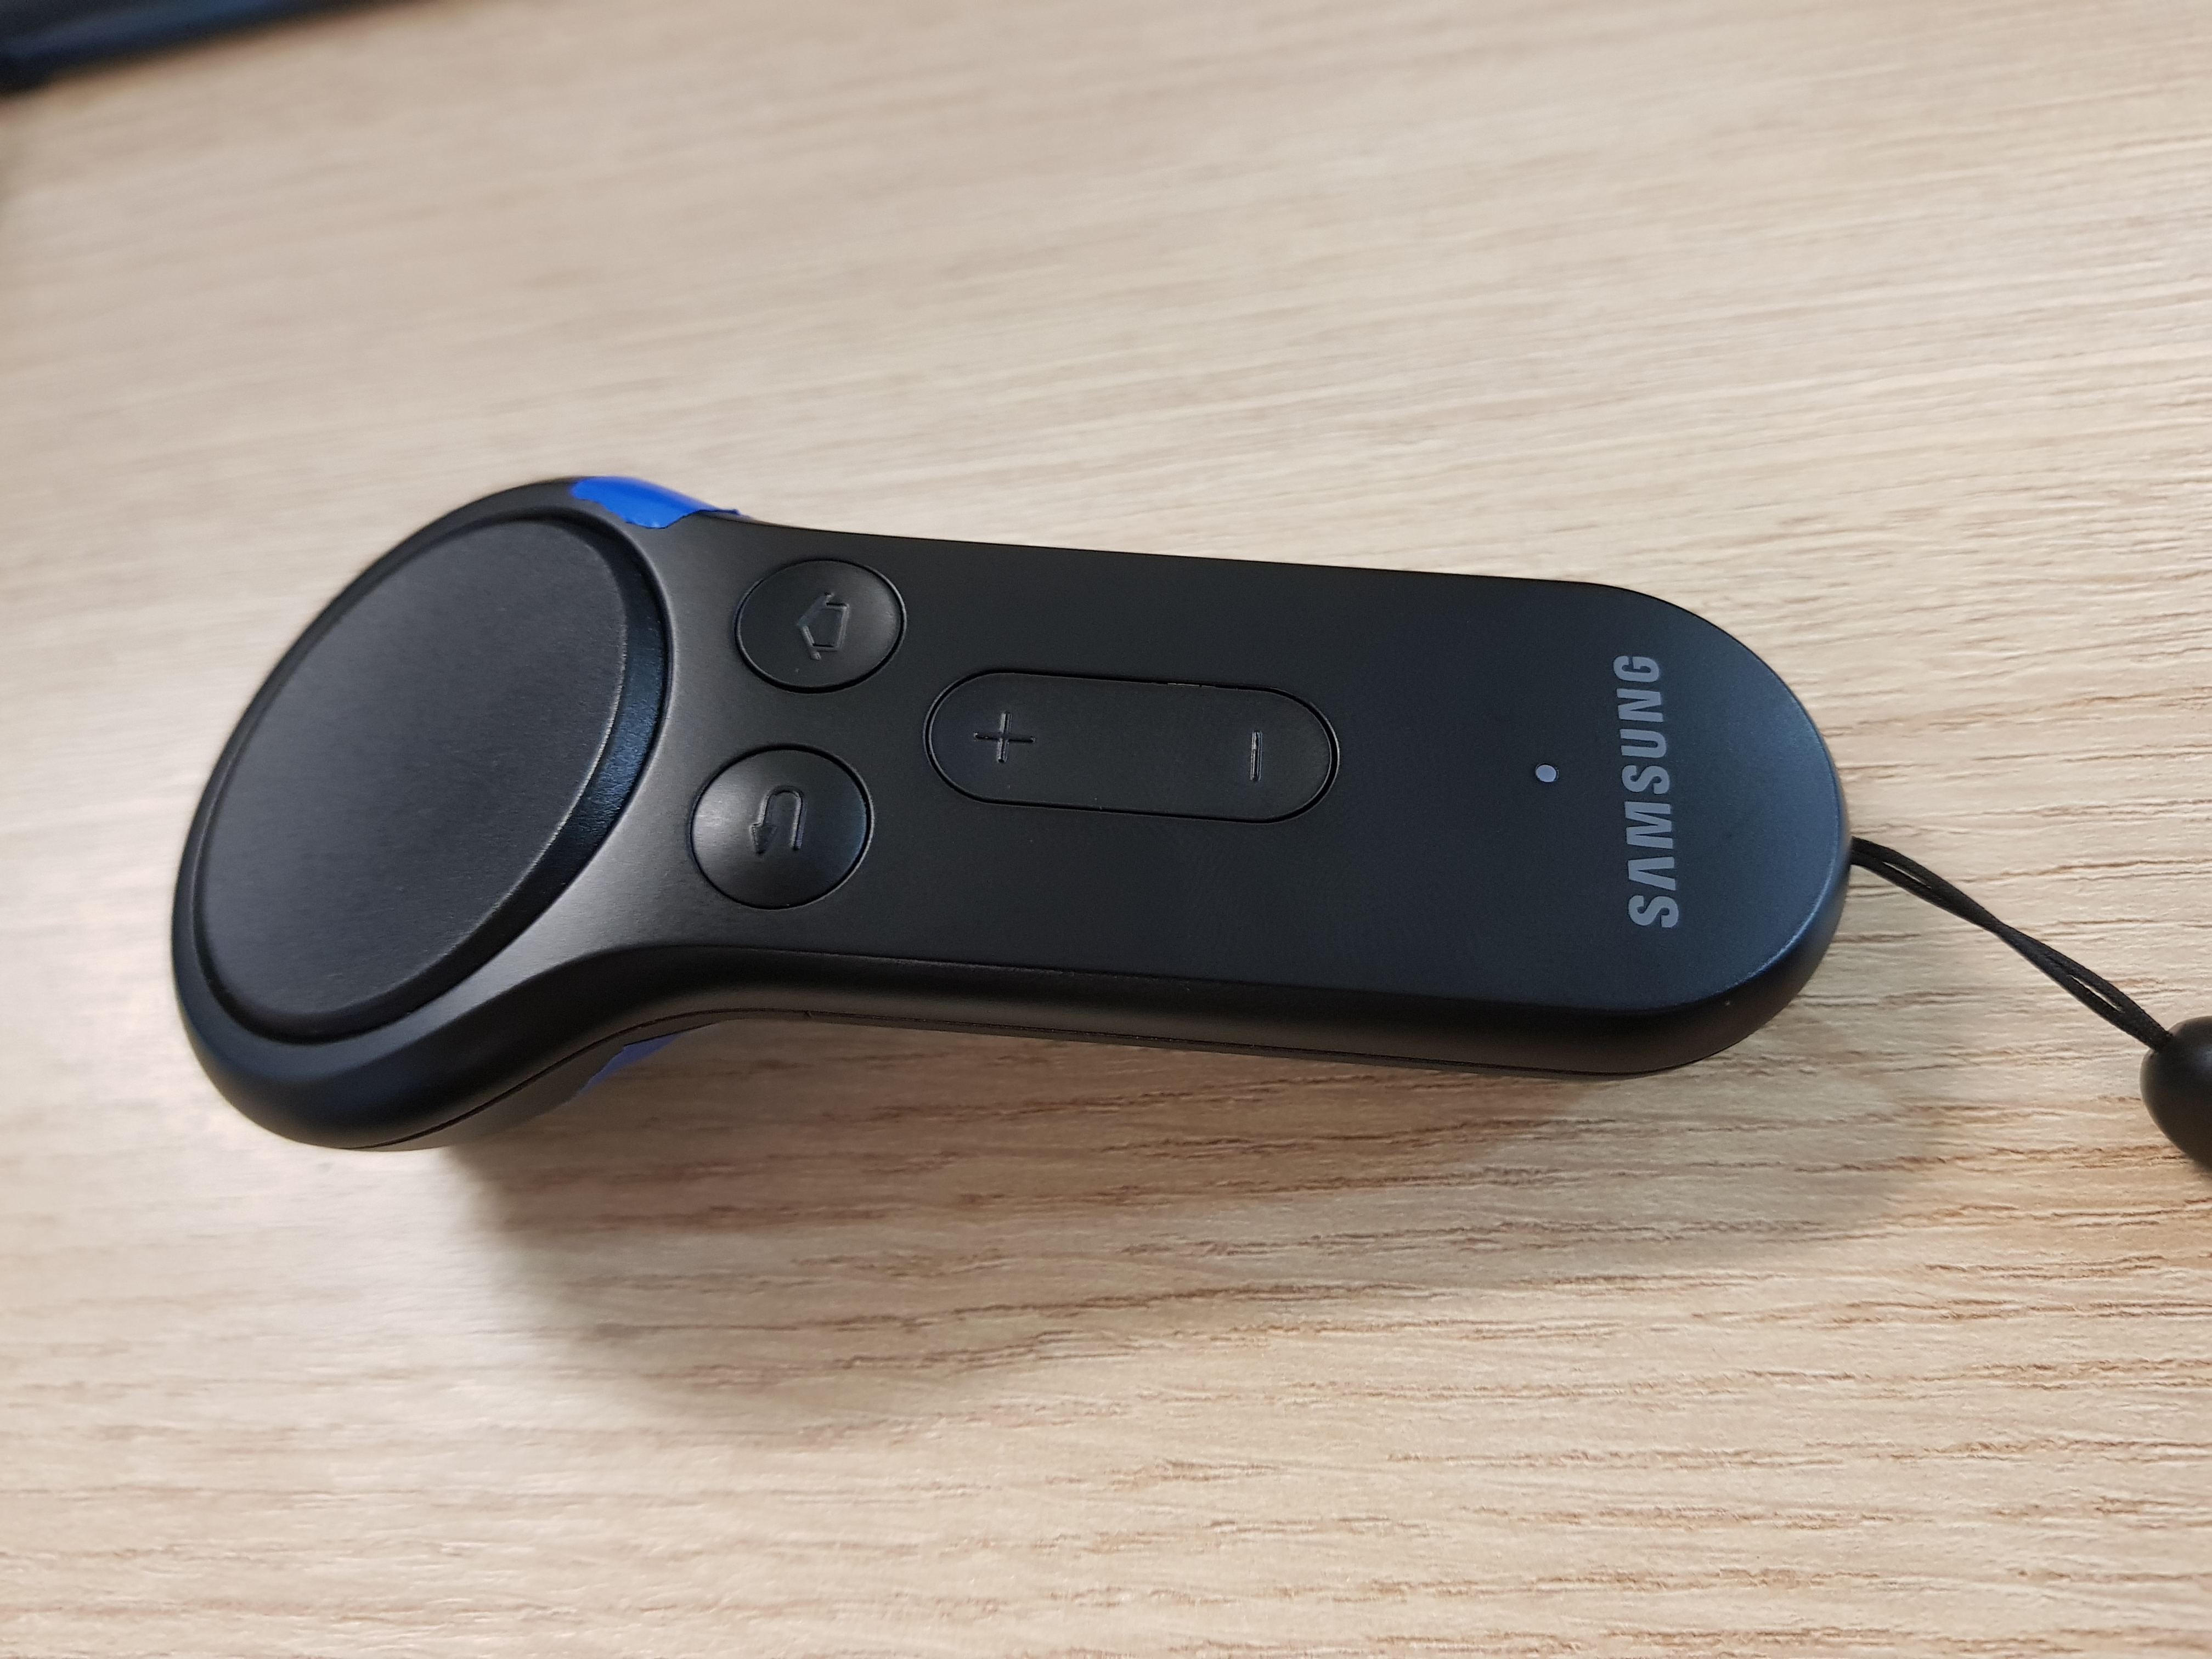
\includegraphics[width=.6\textwidth]{images/gear_controller.jpg}
\caption{Controle para Realidade Virtual da Samsung.}
\label{fig:vrcontroller}
\end{figure}

% * Qual a importância/valor de usar controles?
Aplicativos de realidade virtual normalmente são executados dentro de óculos especialmente feitos para a renderização de duas telas, uma para cada olho, conferindo assim a ilusão de profundidade em um universo virtual, maximizando a imersão do usuário. Em aplicações de realidade virtual, normalmente o controle posiciona um cursor que representa o foco de interação do usuário.

% * Tipos de Controles
Há variações no que se refere às capacidades dos diferentes tipos de controle, o próprio headset, i.e. o equipamento de realidade virtual vestível, possui um controle baseado no giroscópio; existem também controladores que fornecem informações posicionais, permitindo um maior nível de liberdade para o usuário, visto que há a possiblidade de manipulação de diferentes elementos, além da movimentação do próprio personagem do usuário.

% * Descrever controle da Samsung
A figura \ref{fig:vrcontroller} mostra o controle que acompanha o óculos de realidade virtual \textit{GearVR SM-R324} da Samsung. A \textit{Oculus} é atualmente parceira da Samsung na distribuição de soluções para realidade virtual através de dispositivos móveis e disponibiliza um \textit{SDK} para uso de funcionalidades específicas em aplicações de realidade virtual, dentre elas uma API para captação dos dados de rotação do controle \cite{gearvrinputdocs}.


% * Problemas/Imprecisão



\section{Ferramenta de Visualização de Filtros} \label{sec:viztool}

% Proposal
Este artigo se propõe a implementar uma ferramenta para a visualização do emprego do filtro de Kalman na estabilização de um controle de realidade virtual. O uso do filtro é motivado pela necessidade de remoção dos ruídos de leitura e obtenção de um controle mais estável para o usuário. A contribuição para o desenvolvedor é a capacidade de visualizar o efeitos do ruído e compreender como este pode ser amenizado pelo uso do filtro de Kalman; para o usuário final, a criação de um componente para controle de realidade virtual que possibilite movimentos mais precisos.


% As a didatic tool
Dado o objetivo de remover ruídos de um conjunto determinado de sinais, é de grande interesse para o desenvolvedor assimilar de que forma este ruído potencialmente afeta uma aplicação em realidade virtual: principalmente através da geração de um cursor mais trêmulo, menos responsivo ou confiável, dificultando, portanto, a experiência do usuário.


% Describe Unity implementation - Noise visualization
Para visualizar o ruído, utilizou-se elementos de partículas ou \textit{ParticleSystem} para renderizar pontos onde o cursor deveria estar levando em conta as entradas ruidosas tais como recebidas pelo controle. As partículas geradas foram configuradas para ter uma cor destoante, uma tonalidade de vermelho indica a entrada real obtida pelo controle e, ao longo do tempo, reduz-se a luminosidade das partículas de modo a adicionar uma informação temporal à visualização gerada. Assim, pontos vermelhos mais vivos indicam os dados mais recentes recebidos pelo controle enquanto pontos mais fracos representam posições mais antigas.

Afim de comparar a entrada ruidosa e o resultado filtrado, as posições filtradas pelo filtro de Kalman foram destacadas em azul, através de \textit{TrailRenderer} que permite renderizar o caminho percorrido pelo cursor ao longo da execução da aplicação.

\begin{figure}[ht]
\centering
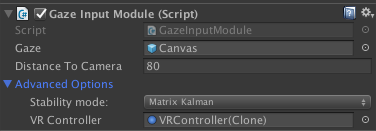
\includegraphics[width=.5\textwidth]{images/controller_input.png}
\caption{Componente Unity para configuração do controle da Samsung.}
\label{fig:controllercomponent}
\end{figure}

% Describe Unity implementation - GearVRInput component
Implementamos um componente de gerenciamento de entradas do usuário chamado \textit{GazeInputModule}, permitindo mudar o cursor de acordo com a posição da cabeça do usuário fornecida pelo \textit{headset GearVR} ou pela rotação do controle.


% Describe interaction with controller
O controle de realidade virtual da Samsung, tal como descrito na seção \ref{sec:vrcontroller}, possibilita obter dados de rotação em tempo real \cite{gearvrinputdocs} na forma de um \textit{quaternion} \cite{quaternionhamilton1844ii} que representa a orientação atual do dispositivo. \textit{Quaternions} são um sistema numérico que estendem os números complexos e são utilizados por muitas \textit{APIs} gráficas para representar valores de rotação. O \textit{Software Development Kit} SDK da \textit{Oculus} permite obter a rotação em coordenadas angulares (ângulos de Euler). Para cada valor angular é calculado um ponto do cursor que intercepta uma esfera de tamanho unitário e um raio partindo da representação virtual do controle.


\section{Resultados} \label{sec:results}

\begin{figure}[ht]
\centering
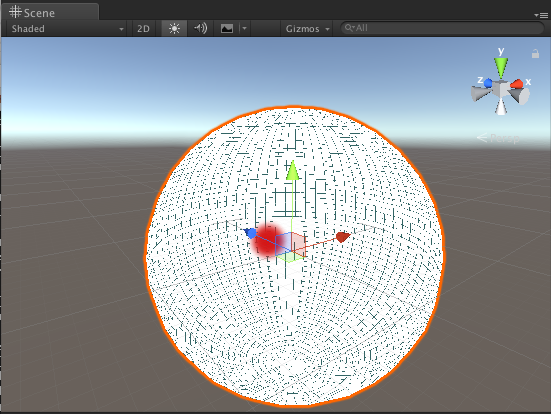
\includegraphics[width=.5\textwidth]{images/sphere.png}
\caption{Esfera invertida na cena da Unity.}
\label{fig:invertsphere}
\end{figure}

A implementação em Unity3D foi executada em um aparelho Samsung S8 acoplado ao óculos \textit{GearVR SM-R324}. Utilizou-se o controle oficial da Samsung, que acompanha o óculos de realidade virtual \textit{GearVR}. Para fins de teste, foi gerada uma esfera invertida e um código em \textit{shader} para exibir \textit{grids} na superfície da esfera gerando um ambiente branco de cor sólida e sem efeitos de iluminação, tal como exibida na figura \ref{fig:invertsphere}.

Toda aplicação \textit{GearVR} distribuída na \textit{Oculus Store} \cite{gearvrstore} pode ser executada nos modelos de celulares Samsung mais avançados, quando acoplado a um óculos \textit{GearVR}. A qualquer momento durante a execução da aplicação, é possível acessar um menu de opções que permite registrar \textit{screenshots} ou gravar vídeos da experiência vivida pelo usuário no mundo virtual estabelecido pela aplicação.

\begin{figure}[ht]
\centering
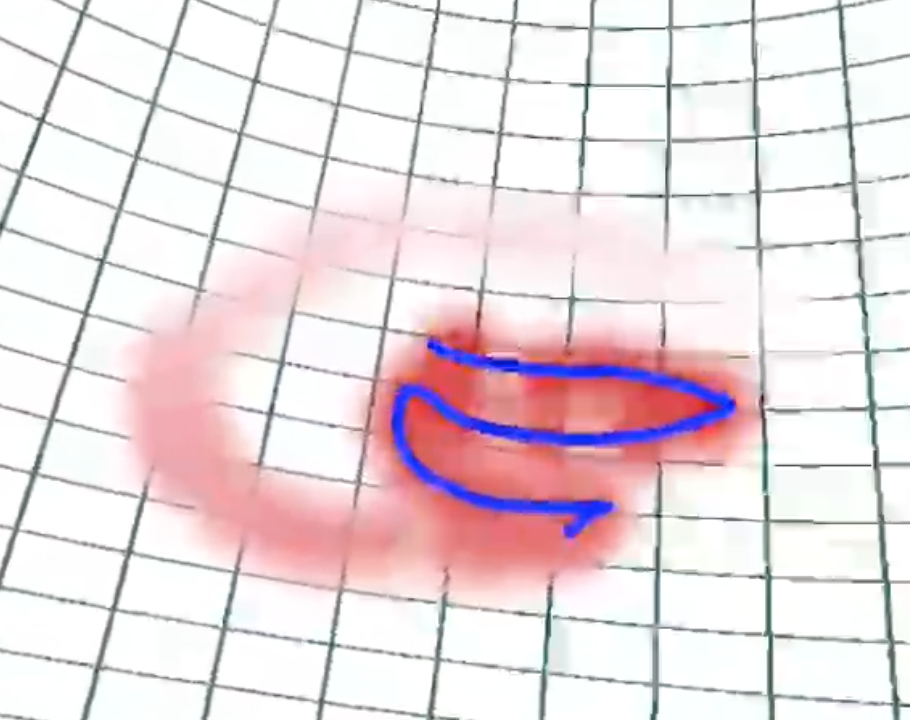
\includegraphics[width=.5\textwidth]{images/image_01.png}
\caption{Filtragem do cursor de VR. Amostras ruidosas em vermelho e valor filtrado em azul.}
\label{fig:filter01}
\end{figure}

A figura \ref{fig:filter01} mostra um \textit{screenshot} da aplicação em Realidade Virtual com a filtragem de cursor ativa. O caminho do cursor é definido pela rotação atual do controle do \textit{GearVR}. A posição do cursor é calculada na intersecção de uma esfera de tamanho unitário e a direção atual do controle.

\begin{figure}[ht]
\centering
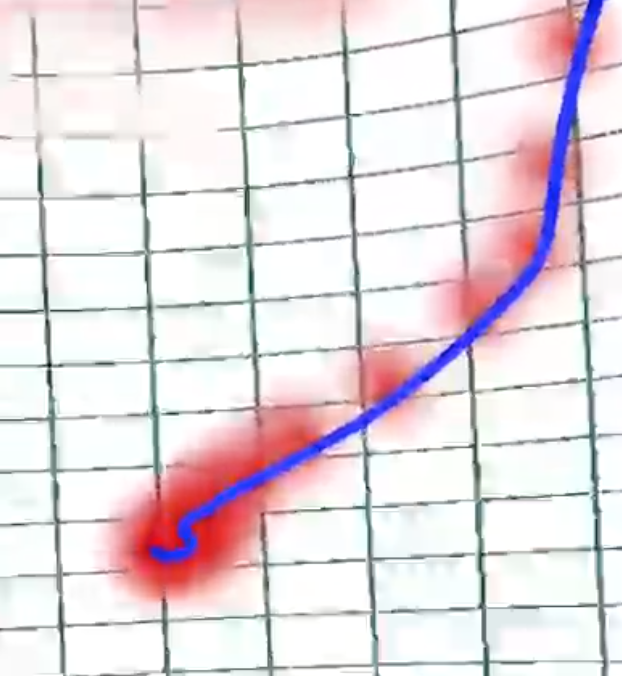
\includegraphics[width=.5\textwidth]{images/image_02.png}
\caption{Filtragem do cursor de VR. Amostras ruidosas em vermelho e valor filtrado em azul.}
\label{fig:filter02}
\end{figure}

Durante a execução da aplicação, percebeu-se que quando a movimentação do cursor é mais veloz que a taxa de atualização, i.e., o \textit{update}, os pontos de ruído não são visualizados de maneira contínua, provocando o efeito visto na figura \ref{fig:filter02}, onde as partículas concentram-se em apenas alguns pontos amostrados pelo \textit{framerate} da aplicação \textit{Unity}, gerando regiões ruidosas espaçadas entre si.

Na figura \ref{fig:filter01} e \ref{fig:filter02} verifica-se que a linha azul forma-se de maneira estável ao longo do caminho percorrido pelo cursor, enquanto os pontos vermelhos se espalham ao redor desse caminho, indicando que a amplitude máxima de instabilidade é cerca de duas vezes maior que o tamanho do cursor, ou seja, facilmente perceptível pelo usuário e que impossibilitaria a realização de movimentos precisos e estáveis, em outras palavras, a exatidão e responsividade esperadas do controlador não são satisfatórias.

\section{Conclusão} \label{sec:conclusion}

Apresentou-se neste artigo uma implementação do filtro de Kalman para estabilização do controle de realidade virtual da Samsung. Concomitantemente, descreveu-se a visualização das entradas ruidosas fornecidas pelo controle e o efeito resultante após a aplicação do filtro de Kalman. Afim de estimular a reutilização da implementações feitas, foram gerados componentes para rápida configuração, tal como demonstrado na figura \ref{fig:controllercomponent}.


Através resultados obtidos, verificou-se que a solução desenvolvida em \textit{Unity} foi capaz de filtrar as posições ruidosas geradas pelo controlador e garantir um nível de controle mais estável em aplicações de realidade virtual. Implementou-se também uma ferramenta para visualização da filtragem de entradas ruidosas.


Em trabalhos futuros propõe-se estender a aplicação do filtro à problemas de outras naturezas, tais quais em aplicações onde haja \textit{jittering} na movimentação de personagens ou ainda em aplicações de realidade aumentada para os mais diversos fins, como garantir que a movimentação de um \textit{non-playable character} (NPC) seja a mais suave possível.


Fora do campo da aplicações digitais, há muitos exemplos possíveis para a aplicação:  um pequeno robô de jardim que precisa saber sua verdadeira localização a fim de evitar quedas; um mapa de navegação para carros que, dentro de um túnel, precise cumprir sua função com precisão para guiar o motorista; ou ainda, a necessidade de conhecer-se a temperatura de um foguete cujo alto aquecimento impeça a medição direta através de um sensor. Se analisadas com cadência, as situações ilustradas possuem em comum a existência de informações que são passíveis de ruídos ou imprecisão os quais podem ser minimizados com o uso do filtro de Kalman.

\section*{Acknowledgment}

The preferred spelling of the word ``acknowledgment'' in America is without 
an ``e'' after the ``g''. Avoid the stilted expression ``one of us (R. B. 
G.) thanks $\ldots$''. Instead, try ``R. B. G. thanks$\ldots$''. Put sponsor 
acknowledgments in the unnumbered footnote on the first page.

\bibliographystyle{IEEEtran}
\bibliography{references}

% \begin{thebibliography}{00}
% \bibitem{b1} G. Eason, B. Noble, and I. N. Sneddon, ``On certain integrals of Lipschitz-Hankel type involving products of Bessel functions,'' Phil. Trans. Roy. Soc. London, vol. A247, pp. 529--551, April 1955.
% \bibitem{b2} J. Clerk Maxwell, A Treatise on Electricity and Magnetism, 3rd ed., vol. 2. Oxford: Clarendon, 1892, pp.68--73.
% \bibitem{b3} I. S. Jacobs and C. P. Bean, ``Fine particles, thin films and exchange anisotropy,'' in Magnetism, vol. III, G. T. Rado and H. Suhl, Eds. New York: Academic, 1963, pp. 271--350.
% \bibitem{b4} K. Elissa, ``Title of paper if known,'' unpublished.
% \bibitem{b5} R. Nicole, ``Title of paper with only first word capitalized,'' J. Name Stand. Abbrev., in press.
% \bibitem{b6} Y. Yorozu, M. Hirano, K. Oka, and Y. Tagawa, ``Electron spectroscopy studies on magneto-optical media and plastic substrate interface,'' IEEE Transl. J. Magn. Japan, vol. 2, pp. 740--741, August 1987 [Digests 9th Annual Conf. Magnetics Japan, p. 301, 1982].
% \bibitem{b7} M. Young, The Technical Writer's Handbook. Mill Valley, CA: University Science, 1989.
% \end{thebibliography}
% \vspace{12pt}
% \color{red}
% IEEE conference templates contain guidance text for composing and formatting conference papers. Please ensure that all template text is removed from your conference paper prior to submission to the conference. Failure to remove the template text from your paper may result in your paper not being published.

\end{document}
